\problemname{Begränsningsarea}

\begin{figure}
\centering
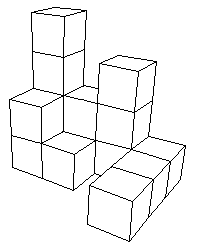
\includegraphics{area}
\end{figure}

Betrakta den tredimensionalla figuren ovan. Den är ihopsatt av ett antal $1 \times 1 \times 1$ kuber i ett 3d-rutnät. Om vi begränsar oss till figurer som har staplar fästa i ``marken'', kan figuren på bilden beskrivas genom att ange höjden för varje stapel: 

\begin{verbatim}
4	2	3	1
2	1	0	1
0	0	0	1
\end{verbatim}

Figurens volym är förstås enkel att beräkna, men här är vi intresserade av dess begränsningsarea, d.v.s. antalet 1x1 kvadrater som är synliga utifrån (inklusive underifrån). Skriv ett program som beräknar detta, givet beskrivningen av en figur. 

\section*{Indata}
På första raden står två heltal $r$ och $k$ ($1 \le r, k \le 50$). Sedan följer $r$ rader med $k$ heltal på varje rad:
höjden $h$ ($0 \leq h \leq 50$) för varje stapel.

\section*{Utdata}
Skriv ut ett heltal: figurens begränsningsarea.

\section*{Poängsättning}
Din lösning kommer att testas på en mängd testfallsgrupper.
För att få poäng för en grupp så måste du klara alla testfall i gruppen.


\noindent
\begin{tabular}{| l | l | p{12cm} |}
  \hline
  \textbf{Grupp} & \textbf{Poäng} & \textbf{Gränser} \\ \hline
  $1$    & $30$       & $h$ är antingen $0$ eller $1$. \\ \hline
  $2$    & $70$       & Inga ytterligare begränsningar. \\ \hline
\end{tabular}
